\subsection{Tissue target avoidance (GTEx): conserved targets avoid the miRNA's tissue, CNN non-conserved targets do not}
Targets of a tissue-specific miRNA should be relatively depleted in that tissue. We test this with GTEx v8 gene median TPM (\texttt{scripts/gtex\_target\_avoidance.py}; \texttt{results/gtex\_target\_avoidance.json}; hermetic tests) on 8 pre-registered pairs (miR-1-3p, miR-133b, miR-206: skeletal muscle; miR-122-5p: liver; miR-9-5p, miR-128-3p: brain cortex; miR-223-3p: whole blood; miR-375: pancreas). Relative expression is $r_g(t)=\log_2(\mathrm{TPM}_{g,t}+1)-\mathrm{median}_{t'}\log_2(\mathrm{TPM}_{g,t'}+1)$ and depletion is the Mann--Whitney probability $\mathrm{AUC}_{dep}=P(r_{\text{set}}<r_{\text{rest}})$. Gates passed: ALB peaks in liver, ACTA1 in skeletal muscle, median mapping 95.6\%.
CNN top-200 genes are not depleted in the matched tissue (H1: 1 wins, 7 losses, $p=0.996$) and not more depleted there than in the other design tissues (H3: 5/3, $p=0.363$); both are falsified. Pre-registered H2 (TargetScan genes inside the CLIP universe) turned out to be empty by construction, since that universe excludes every gene with a conserved site for the seed; we record it as not evaluable. A post-hoc reference arm that we did not pre-register uses all TargetScan 3'UTR genes as the universe and the top-200 conserved-site genes as the set: they are depleted in the matched tissue for 8/8 pairs ($p=0.004$) and more so than in other tissues for 7/8 ($p=0.035$; Figure~\ref{fig:gtex}), which recovers the classic avoidance signal (Farh et al.\ 2005).
So the method sees avoidance where it is expected, and the CNN's non-conserved candidates show none. Two caveats: the arms use different universes (CNN scores exist only for the CLIP universe), and conservation and scorer are confounded, so this does not separate ``non-conserved sites are not functional in vivo'' from ``the CNN ranks them poorly.'' Both readings are negative for the non-conserved discovery claim.
\begin{figure}[h]\centering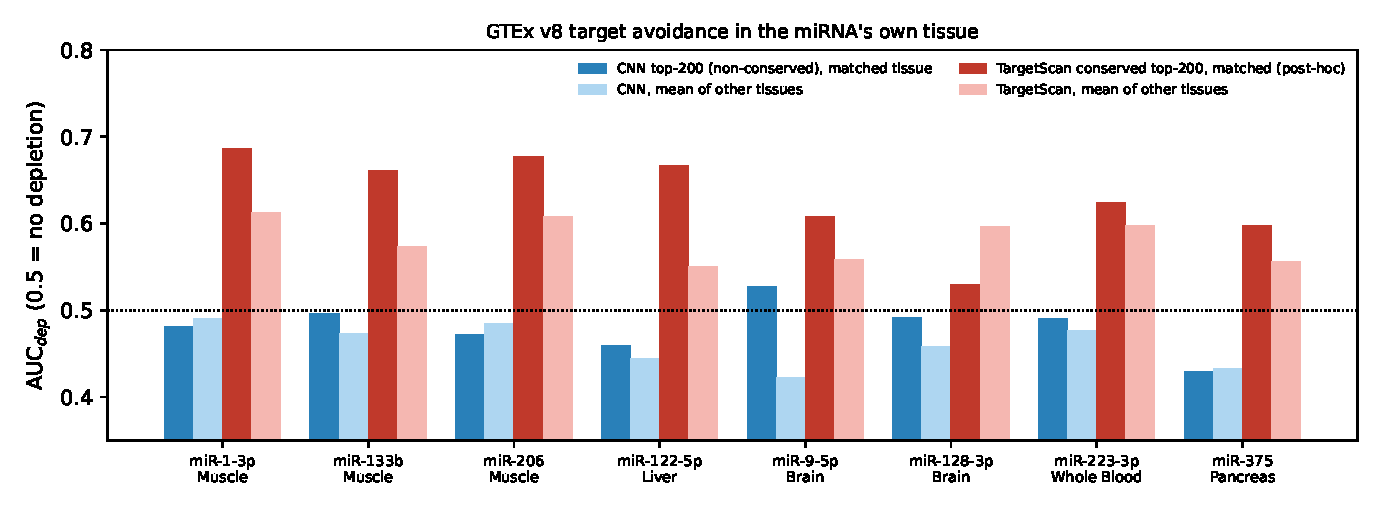
\includegraphics[width=0.95\linewidth]{figs/fig_gtex.pdf}
\caption{Depletion (AUC$_{dep}$) of target sets in each miRNA's own GTEx tissue versus the mean over the other design tissues. Blue: CNN top-200 in the CLIP universe (pre-registered). Red: TargetScan conserved top-200 in the all-UTR universe (post-hoc reference).}\label{fig:gtex}\end{figure}
